%!LW recipe=latexmk (xelatex)
%!TEX program = xelatex
%LTex: enabled=true

\documentclass{article}

\title{\bfseries Humidity Measurements\\ from Weather Stations\\ at OAN}
\author{Alan M. Watson}
\date{4 October 2025}

\usepackage{plex-otf}
\usepackage{unicode-math}
\setmathfont{IBM Plex Math}

%\usepackage{fullpage}
\usepackage{graphicx}

\setlength{\parskip}{0.8ex plus 0.3ex}
\setlength{\parindent}{0ex}

\begin{document}

\maketitle

\begin{abstract}

    \setlength{\parskip}{0.8ex plus 0.3ex}
    \setlength{\parindent}{0ex}
    \noindent

    The COLIBRÍ weather station has been observed to give humidity readings that are often of order 10\% lower than those of the OAN weather stations.  To understand this,  have compared the humidity readings of the COLIBRÍ, BOOTES-5, and OAN weather stations during a period of relatively humid weather.
    
    The COLIBRÍ station never gave a reading higher than 90\%, despite the observed presence of fog and rain, indicating that the differences between the COLIBRÍ and OAN stations cannot simply be attributed to their different locations. Comparison to the OAN stations suggests that the COLIBRÍ station has a calibration offset of about 14\%. 
    
    The BOOTES-5 station seems to suffer a similar but smaller offset of about 5\%.

\end{abstract}

\section{Context}

The OAN and COLIBRÍ operations teams have remarked recently that the COLIBRÍ weather station gives humidity readings that are often of order 10\% lower than those of the OAN weather stations. 

Some of this might be due to the differences in location, as the COLIBRÍ weather station is on a tall mast at the very top of the summit and the OAN stations are near to the Johnson telescope at a lower level. While location undoubtedly plays some role, the COLIBRÍ operations team has noticed events in which fog blowing by the telescope is seen on the external webcam, but the humidity reading is below 80\%. This suggests an error in the absolute calibration.

I therefore have compared the COLIBRÍ, BOOTES-5, and OAN weather stations to attempt to understand this issue.

\section{Data}

I have collected data from four weather stations on the main summit at the OAN:

\begin{itemize}

\item The COLIBRÍ station. This station is located at the top of the six-meter mast shared by COLIBRÍ and BOOTES-5. It is a Vaisala station.

\item The BOOTES-5 station. This station only takes measurements at night. It is located about half-way up the six-meter mast shared by COLIBRÍ and BOOTES-5. The data for this station were kindly provided by Alberto Castro-Tirado and Emilio Fernández-García.

\item The two OAN stations, which I designate A and B. 

Station A is to the west of the Johnson telescope, and its data are available at 132.248.4.66. 

Station B is on the very tall mast on the rocks between the 84-cm and Johnson telescopes, and its data are available at 132.248.4.141.

\end{itemize}

\begin{figure}
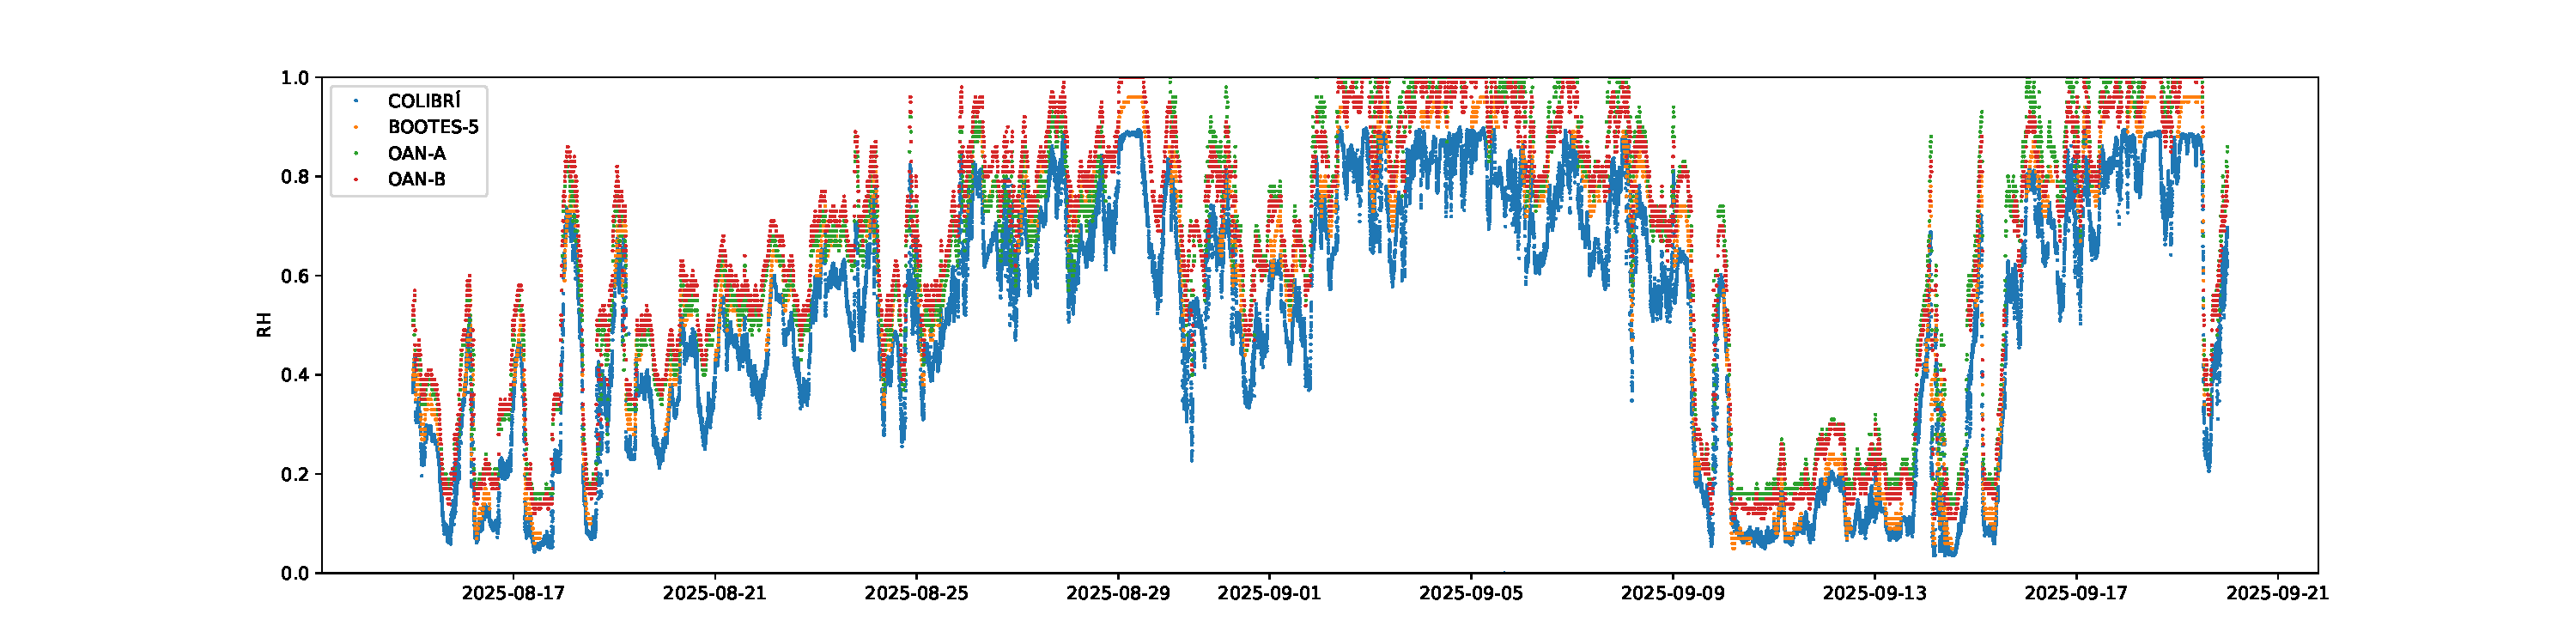
\includegraphics[width=\linewidth]{humidity-all.pdf}
\caption{
    The relative humidity measurements from the COLIBRÍ (blue), BOOTES-5 (yellow), OAN-A (green), and OAN-B (blue) stations in the second half of 2025 August and most of 2025 September.
}
\label{figure:humidity-all}
\end{figure}


\section{Analysis}

Figure~\ref{figure:humidity-all} shows the relative humidity for the second half of 2025 August and most of 2025 September for these stations. This period was chosen as it shows several episodes of very high humidity, which is the most important regime for telescope safety.

The figure shows that there are systematic offsets between the stations. COLIBRÍ tends to give a lower reading than BOOTES-5, and BOOTES-5 tends to give a lower reading than the OAN stations.

Moreover, we had several days and nights with fog and rain during this period. Despite this, the highest relative humidity reading was 89.9\% for the COLIBRÍ station and 96\% for BOOTES-5, whereas it was 100\% for the OAN stations. That the COLIBRÍ station never read higher than 90\% strongly suggests that it is not reading the correct humidity but instead has an offset or is saturating.

\begin{figure}
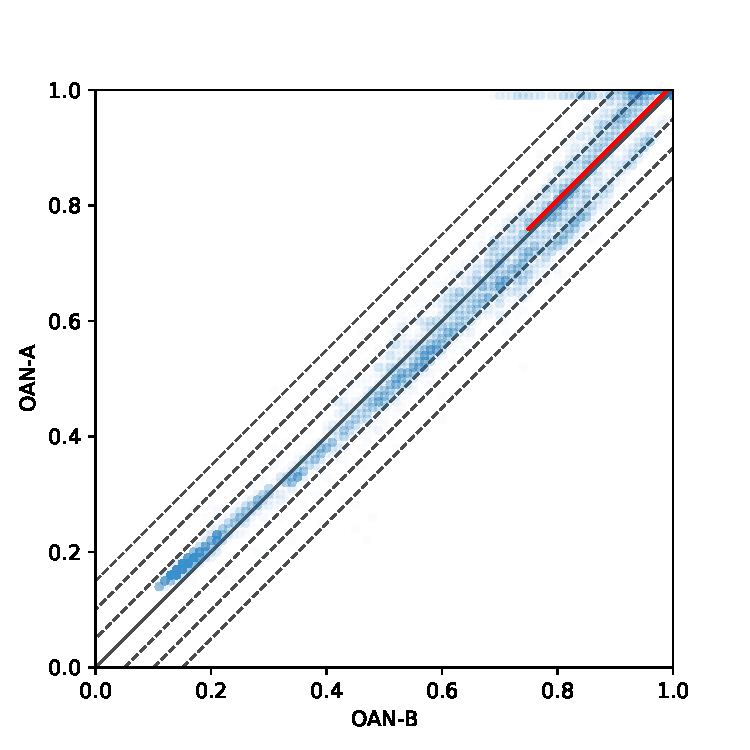
\includegraphics[width=\linewidth]{humidity-correlation-OAN-B-OAN-A.pdf}
\caption{
    The differences in humidity measurements from the OAN-B and OAN-A stations in the second half of 2025 August and most of 2025 September. The red line shows the median offset of $+1\%$ between humidities of 75\% and 100\%. 
}
\label{figure:humidity-OAN-B-OAN-A}
\end{figure}

\begin{figure}
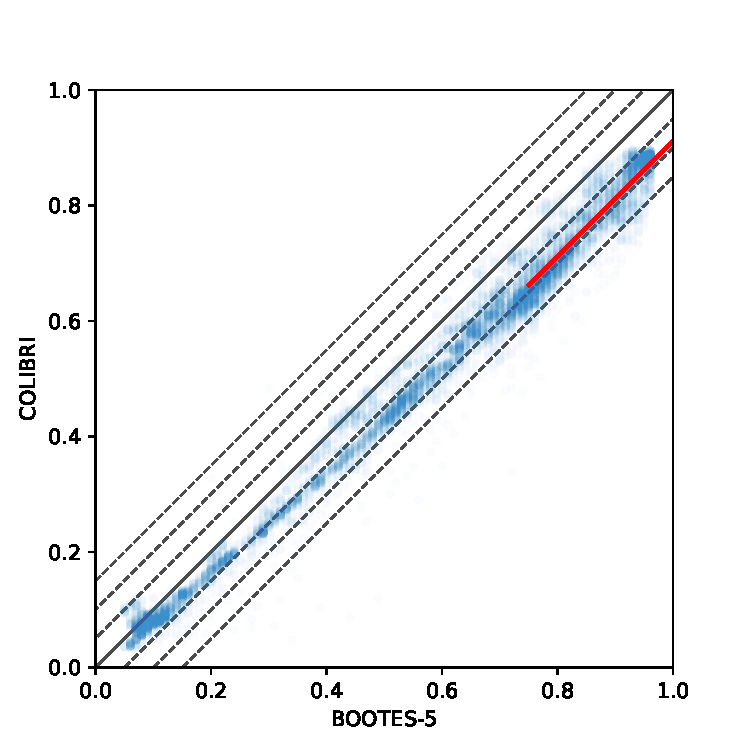
\includegraphics[width=\linewidth]{humidity-correlation-BOOTES-5-COLIBRI.pdf}
\caption{
    The differences in humidity measurements from the BOOTES-5 and COLIBRÍ stations in the second half of 2025 August and most of 2025 September. The red line shows the median offset of $-9\%$ between humidities of 75\% and 100\%. Notice that neither station ever reads 100\% in this period, despite observed episodes of fog and rain.
}
\label{figure:humidity-BOOTES-5-COLIBRI}
\end{figure}

\begin{figure}
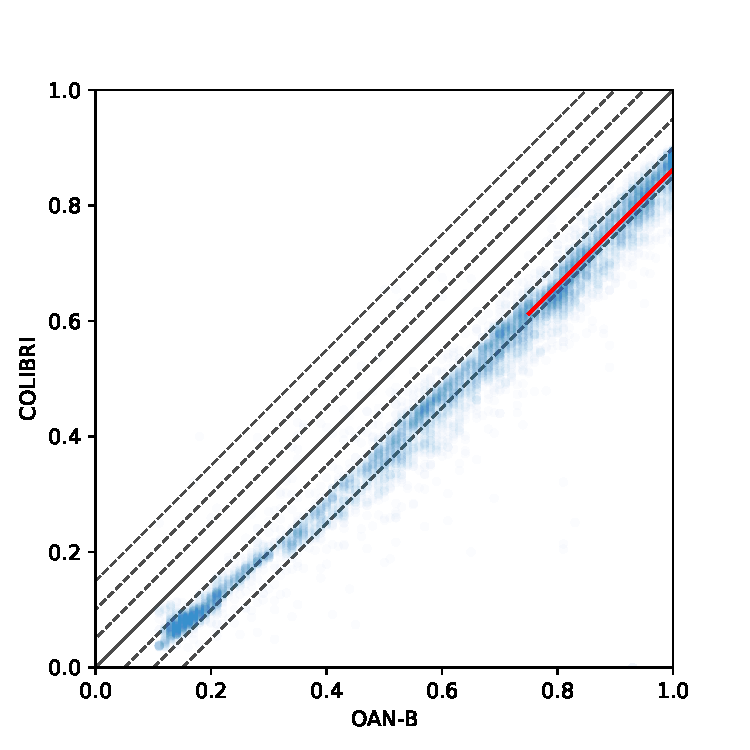
\includegraphics[width=\linewidth]{humidity-correlation-OAN-B-COLIBRI.pdf}
\caption{
    The differences in humidity measurements from the OAN-B and COLIBRÍ stations in the second half of 2025 August and most of 2025 September. The red line shows the median offset of $-14\%$ between humidities of 75\% and 100\%. 
}
\label{figure:humidity-OAN-B-COLIBRI}
\end{figure}

\begin{figure}
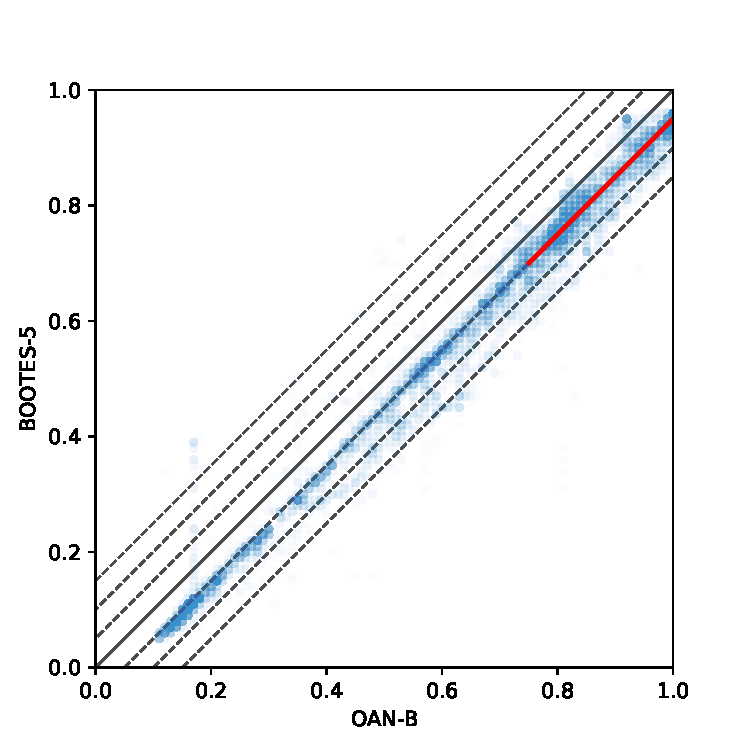
\includegraphics[width=\linewidth]{humidity-correlation-OAN-B-BOOTES-5.pdf}
\caption{
    The differences in humidity measurements from the OAN-B and BOOTES-5 stations in the second half of 2025 August and most of 2025 September. The red line shows the median offset of $-5\%$ between humidities of 75\% and 100\%. 
}
\label{figure:humidity-OAN-B-BOOTES-5}
\end{figure}

A better understanding can be gained by plotting simultaneous values of humidity:

\begin{itemize}

\item 
Figure \ref{figure:humidity-OAN-B-OAN-A} shows the readings of the OAN-B and OAN-A stations. At high humidities (75\% to 100\%) there is an offset of about 1\% between them. That said, there is considerable scatter, with station A sometimes showing 100\% humidity while station B has much lower humidities. This may be a local effect, as station A is located next to trees and station B is in free air.

\item 
Figure \ref{figure:humidity-BOOTES-5-COLIBRI} shows the readings of the BOOTES-5 and COLIBRÍ stations. At high humidities (75\% to 100\%) there is an offset of about 9\% between them. As previously mentioned, neither station ever read 100\% in this period, despite observed episodes of fog and rain. This suggests that we cannot simply use the BOOTES-5 station to correct the COLIBRÍ station, as both show unusual behavior.

\item 
Figure \ref{figure:humidity-OAN-B-COLIBRI} shows the readings of the OAN-B and COLIBRÍ stations. At high humidities (75\% to 100\%) there is an offset of about 14\% between them. The form of the relation suggests an offset rather than a saturation effect. The offset would appear to be at least 10\%, the value required to take the maximum reading of 89.9\% to almost 100\%, but the comparison to the OAN-B station suggests that it is closer to 14\%.

\item 
Figure \ref{figure:humidity-OAN-B-BOOTES-5} shows the readings of the OAN-B and BOOTES-5 stations. At high humidities (75\% to 100\%) there is an offset of about 5\% between them. Again, the form of the relation suggests an offset rather than a saturation effect.

\end{itemize}

\section{Actions}

In the short term, the COLIBRÍ operations team propose in the short term to add 14\% to the measurements of the COLIBRÍ station in order to adjust it to the same scale as the OAN-B station. 

In the longer term, they are interested in recalibrating their station.

\end{document}
